\chapter{GÉNÉRALITÉ SUR L'INTELLIGENCE ARTIFICIELLE}
\begin{spacing}{1.2}
\minitoc
\thispagestyle{MyStyle}
\end{spacing}
\newpage

L'intelligence artificielle (IA) a connu une évolution rapide ces dernières années, s'imposant comme une force majeure dans notre société. Son influence s'étend à tous les aspects de notre vie quotidienne, de la santé à l'éducation en passant par les loisirs. De plus en plus, nous voyons l'IA jouer un rôle crucial dans l'amélioration de l'efficacité, la prise de décisions éclairées et la création d'expériences personnalisées pour les individus. Toutefois, l'IA est un domaine vaste et complexe, qui englobe différentes approches et techniques pour simuler l'intelligence humaine. Dans ce chapitre, nous explorerons l'IA et son avenir en passant par ses fondements.

\section{Exploration de l'intelligence artificielle}
\subsection{Historique}

Des machines destinées à simuler les comportements humains ont été imaginées bien avant la création de la robotique et de l’informatique aux XVIIIe et XIXe siècles. Mais il s’agissait alors d’automates, dont chaque action, ou chaque réaction dans un contexte donné, devait être préalablement pensée et intégrée explicitement dans des mécanismes complexes \cite{boisard2020}.
Au XXe siècle, \textbf{Alan Turing} a notamment inventé un modèle de calcul par la suite appelé \textit{machine de Turing}, exploré la notion de calculabilité et d'intelligence des machines, et proposé le « jeu de l'imitation » (test de Turing\textsuperscript{}) \footnote{\textbf{Test de Turing} est une proposition de test d’intelligence artificielle fondée sur la faculté d'une machine à imiter la conversation humaine.} pour évaluer l'intelligence de futures machines \cite{turing1950}. C'est en 1952 que \textbf{Arthur Samuel}, informaticien américain, a créé son programme pour IBM, dont le programme jouait au jeu de Dames et s'améliorait en jouant. À terme, il parvint à battre le 4e meilleur joueur des États-Unis. Il inventa le terme « machine learning » ( apprentissage automatique ) en 1959 \cite{samuel}. 
\\
Le terme « intelligence artificielle », quant à lui, a été mis en avant par \textbf{John McCarthy} lors de la conférence de Dartmouth en 1956, où l'intelligence artificielle a été établie en tant que discipline à part entière \cite{mccarthy1956}.
\\
Une avancée majeure dans le secteur de l'intelligence machine est le succès de l'ordinateur développé par IBM, Deep Blue\textsuperscript{} \footnote{\textbf{Deep Blue} est un superordinateur spécialisé dans le jeu d'échec.}, qui est le premier à vaincre le champion mondial d'échecs \textbf{Garry Kasparov} en 1997. Le projet Deep Blue en inspirera nombre d'autres dans le cadre de l'IA, particulièrement un autre grand défi : IBM Watson\textsuperscript{} \footnote{\textbf{Watson} est un programme informatique conçu pour répondre à des questions formulées en langage naturel.}, l'ordinateur dont le but est de gagner au jeu Jeopardy!. Ce but est atteint en 2011, quand Watson gagne à Jeopardy! en répondant aux questions par traitement de langage naturel \cite{wiki_ml}.
Dans les années qui ont suivi, des chercheurs ont proposé diverses preuves de concept, dans des situations spécifiques, de ce que les machines peuvent faire en théorie. Autour des années 2000, le Web 2.0, le big data et de nouvelles infrastructures et capacités de calcul ont permis l'exploration de masses de données sans précédent à travers le « Deep learning » : il s'agit des réseaux de neurones profonds qui ont fait leur retour avec des progrès significatifs dans le traitement des données massives et l'apprentissage profond \cite{lecun2015}.
\\
En 2015, une nouvelle étape importante est atteinte lorsque l'ordinateur « AlphaGo\textsuperscript{} \footnote{\textbf{AlphaGo} est un programme informatique capable de jouer au jeu de go.} » de Google gagne contre un des meilleurs joueurs au jeu de Go, jeu de plateau considéré comme le plus dur du monde \cite{wiki_ml}.
\\
En 2022, des programmes générant des images à partir de descriptions textuelles, comme Midjourney ou DALL-E, se sont popularisés, et l'agent conversationnel ChatGPT a affiché une croissance inédite, gagnant un million d'utilisateurs en seulement cinq jours et cent millions d'utilisateurs en deux mois, ce qui a accentué un phénomène de « course » à l'IA. En 2023, les progrès rapides de l'IA ont suscité des inquiétudes quant à un potentiel risque d'extinction de l'humanité.

\begin{figure}[H]%
    \center%
    \setlength{\fboxsep}{5pt}%
    \setlength{\fboxrule}{0.5pt}%
    \fbox{
    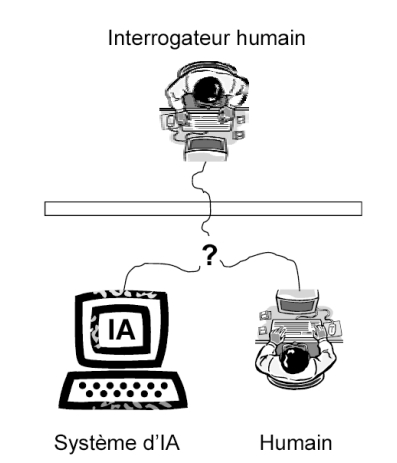
\includegraphics[width=10cm,height=6cm]{images/Test de turing.jpeg}%
    }
    \caption{Test de Turing.}%
\end{figure}

\subsection{Définition}
Selon \textbf{John McCarthy}, l’un des pionniers du domaine, l’IA est « la science et l’ingénierie de la fabrication de machines intelligentes ». C’est un domaine de l’informatique qui cherche à créer des systèmes capables de réaliser des tâches qui nécessiteraient normalement l’intelligence humaine.

Cependant, l’IA est souvent considérée comme un concept vaste et multidimensionnel, difficile à définir précisément en raison de sa nature étendue et en constante évolution.
\\
Elle est également définie par l'un de ses créateurs, \textbf{Marvin Lee Minsky}, comme « la construction de programmes informatiques qui s'adonnent à des tâches qui sont, pour l'instant, accomplies de façon plus satisfaisante par des êtres humains, car elles demandent des processus mentaux de haut niveau tels que : l'apprentissage perceptuel, l'organisation de la mémoire et le raisonnement critique » \cite{Lee}. On y trouve donc le côté « artificiel » atteint par l'usage des ordinateurs ou de processus électroniques élaborés et le côté « intelligence » associé à son but d'imiter le comportement.

\subsection{Classification de l’intelligence artificielle}

La classification de l’intelligence artificielle a pour vocation de permettre la compréhension des différentes catégories de systèmes développés dans ce domaine. Nous proposons ci-dessous les trois types d'IA :
\begin{itemize}  
	\item[\ding{118}]\textbf{L’IA faible}: également connue sous le nom d’IA étroite, elle désigne des systèmes d’IA spécialisés dans une tâche spécifique. Ces systèmes sont conçus pour effectuer une seule tâche de manière très performante, mais ils ne possèdent pas la capacité d’apprentissage ni la compréhension générale du contexte comme le font les humains. Ce qui démontre fort heureusement que l’humain a encore toute sa place dans les tâches et n’est pas prêt à être remplacé par l’IA.
	 
	\item[\ding{118}] \textbf{L’IA forte } : également connue sous le nom d’IA générale, représente un niveau supérieur d’intelligence artificielle. Contrairement à l’IA faible, l’IA forte possède la capacité d’apprendre par elle-même, de comprendre le contexte et de s’adapter à de nouvelles situations. Ainsi, bien que privée de conscience, qui reste quant à elle propre aux organismes vivants, la machine acquiert de l’expérience lui permettant de modifier son propre fonctionnement. Autrement dit, un apprentissage complémentaire découle des tâches qu’elle réalise, ce qui entraîne des réactions initialement non programmées. Ce niveau d’IA est encore largement théorique et n’a pas encore été pleinement atteint, bien que des progrès significatifs aient été réalisés dans le domaine de l’apprentissage automatique et des réseaux neuronaux.
	
	\item[\ding{118}] \textbf{La superintelligence artificielle} : le jour où l’IA dépassera l’intelligence humaine (notamment quand elle aura conscience de son existence) on parlera de superintelligence artificielle. On en est encore loin, mais avec les récentes évolutions très fortes et rapides dont l’humanité a été témoin (par exemple Chat GPT-4), il est légitime de penser que la superintelligence artificielle verra le jour dans le courant du 21e siècle. 
\end{itemize} 

\subsection{Domaines d'application}
L'IA a connu une évolution rapide ces dernières années et a pris une place prépondérante dans notre vie quotidienne. De plus en plus, nous voyons l'intégration de solutions d'IA dans divers aspects de notre vie pour améliorer notre quotidien. Cependant, l'IA est un domaine vaste, et il existe différents domaines d'application adaptés à des besoins spécifiques dans notre vie quotidienne. Dans cette section, nous explorerons ses principaux domaines d'application. 

\subsubsection{La robotique} La robotique a recours à l'IA à plusieurs égards. Notamment pour la perception de l'environnement (objets et visages), l'apprentissage et l'IA développementale. L'interaction homme-robot manque encore souvent de naturel et est un enjeu de la robotique. Il s'agit de permettre aux robots d'évoluer dans le monde dynamique et social des humains et d'échanger avec eux de façon satisfaisante. 

\subsubsection{Le militaire} Le domaine militaire utilise de plus en plus l'IA, notamment pour le pilotage automatique, le guidage de missiles, l'identification, le commandement, l'aide à la décision, la cyberguerre et la cyberdéfense, ou pour la documentation et les processus administratifs. À titre illustratif, confrontés à des missions à risques, les États-Unis se positionnent comme précurseurs de l’intelligence artificielle dans le secteur militaire. Leur production propose des robots autonomes ou télécommandés, pourvus d’une IA, permettant ainsi de remplacer l’Homme en position de combat.
 
\subsubsection{La médecine} Principalement importée de façon robotique, l’IA augmente la croissance de nombreux domaines liés à la technologie. La médecine en est un des exemples les plus concrets depuis 1980, date qui a signé l’apparition des premiers robots de guidage dans les blocs opératoires. Ces derniers permettent grâce à des capteurs de réaliser des mouvements miniaturisés dotés d’une grande précision. La médecine a aussi vu de grands progrès grâce à l'utilisation de systèmes d'aide au diagnostic ou de diagnostic automatisé. \\ C'est dans ce sens que Google DeepMind a également conçu AlphaFold, un système d'IA utilisant l'apprentissage profond qui permet de prédire la façon dont des protéines se replient. 

\subsubsection{Le droit} Le droit fait appel à l'IA dans la perspective de prédire les décisions de justice, d'aider à la décision et de trancher les cas simples. L'Estonie a par exemple développé une intelligence artificielle capable de prendre des décisions de justice sur des délits mineurs. Les États-Unis utilisent par ailleurs dans certaines juridictions le système COMPAS (Correctional Offender Management Profiling for Alternative Sanctions), un système d'aide à la prise de décision pour les juges. 

\subsubsection{Art et littérature} Les IA sont en mesure de produire des compositions musicales imitant le style du compositeur de notre choix. De même, certaines intelligences artificielles peuvent s’approprier le style d’écriture d’un écrivain célèbre et produire une œuvre littéraire qui pourrait très bien compter dans la bibliographie de l’auteur. D’ailleurs, en 2016, un prix littéraire a failli être décerné à une IA japonaise ayant coécrit une nouvelle.

\section{Les domaines de l'intelligence artificielle}
Les domaines de l’IA réside dans une base, qui fait référence aux éléments fondamentaux qui composent la technologie. Ces éléments de base comprennent, entre autres, l’apprentissage automatique, l'apprentissage profond, le traitement du langage naturel et la vision par ordinateur. Ensemble, ces composants forment l’épine dorsale de l’IA, permettant aux machines d’apprendre, de s’adapter et de s’améliorer au fil du temps.

\subsection{L'apprentissage automatique}
L'apprentissage automatique est un sous-ensemble de l'IA qui se concentre sur le développement d'algorithmes permettant aux machines d'apprendre à partir de données et de faire des prédictions ou des décisions sans être explicitement programmées. Par exemple, une plateforme de commerce électronique utilise des algorithmes d’apprentissage automatique pour recommander des produits aux clients en fonction de leur historique de navigation, de leurs achats et de leur historique de recherche. \\
Dans le chapitre suivant, nous verrons en long et en large ce qui est de l'apprentissage automatique.

\subsection{L'apprentissage profond}
L'apprentissage profond, également connu sous sa dénomination anglaise "Deep Learning" (DL), est en effet un cas particulier de l'apprentissage automatique. Il repose sur l'utilisation de réseaux de neurones artificiels, des structures algorithmiques inspirées du fonctionnement du cerveau humain. Ce type d'apprentissage est caractérisé par l'utilisation de 5 couches de neurones ou plus, permettant ainsi de capturer des représentations complexes des données en plusieurs niveaux d'abstraction.

\subsection{Le traitement du langage naturel}
Le traitement du langage naturel (NLP) fait référence à la capacité des machines à comprendre, interpréter et générer le langage humain. La NLP est essentielle pour les chatbots, les assistants virtuels et les systèmes de reconnaissance vocale qui permettent aux utilisateurs d'interagir avec les machines en utilisant le langage naturel.

\subsection{La vision par ordinateur}
La vision par ordinateur implique d’entraîner des machines à interpréter et à comprendre les données visuelles du monde qui les entoure. Grâce à la vision par ordinateur, les machines peuvent reconnaître des objets, des visages et même des émotions, ce qui est essentiel pour des applications telles que la reconnaissance faciale, la surveillance et les voitures autonomes.

\begin{figure}[H]%
    \center%
    \setlength{\fboxsep}{5pt}%
    \setlength{\fboxrule}{0.5pt}%
    \fbox{
    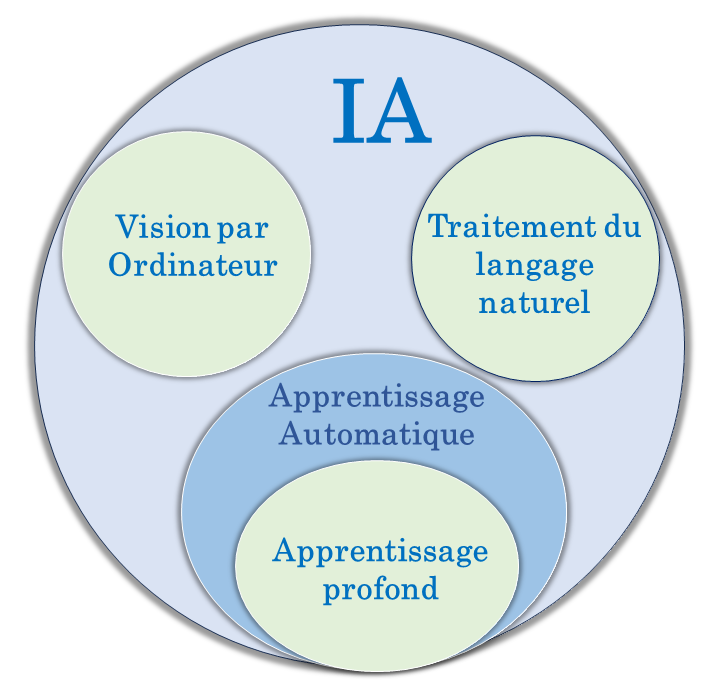
\includegraphics[width=8cm,height=6cm]{images/fondemdent de IA.png}%
    }
    \caption{Fondement de IA.}%
\end{figure}

\section{L'avenir de l'IA et son impact potentiel}
L'IA façonne l'avenir de la technologie et révolutionne notre façon de vivre, de travailler et de communiquer. Les progrès réalisés dans le domaine de l’IA ont transformé la façon dont nous interagissons avec la technologie et les machines, et les possibilités de ce que l’IA peut réaliser sont infinies. Cependant, le potentiel de l’IA s’accompagne également de risques et de défis potentiels qui doivent être surmontés\cite{fastercapital}. Dans cette section, nous discuterons de l’avenir de l’IA et de son impact potentiel sur la société.

\subsection{Le progrès de l’IA }
Les progrès réalisés dans le domaine de l’IA ont été remarquables et la technologie a parcouru un long chemin ces dernières années. Les machines basées sur l’IA peuvent désormais apprendre et s’adapter à de nouvelles situations, effectuer des tâches complexes et même prendre des décisions par elles-mêmes. Les applications potentielles de l’IA sont vastes, depuis les voitures autonomes jusqu’aux soins de santé personnalisés.

\subsection{L'impact sur le marché du travail}
L'essor de l'IA a suscité des inquiétudes quant à son impact sur le marché du travail. Les machines basées sur l’IA peuvent effectuer des tâches qui étaient autrefois effectuées par des humains, ce qui pourrait entraîner des suppressions d’emplois. Cependant, de nombreux experts affirment que l’IA créera de nouveaux emplois et opportunités, et que les humains seront toujours nécessaires pour superviser et entretenir les machines alimentées par l’IA.

\subsection{Les préoccupations éthiques}
L’utilisation de l’IA soulève également des préoccupations éthiques, notamment en ce qui concerne les questions de confidentialité et de préjugés. Par exemple, les systèmes basés sur l’IA qui utilisent la technologie de reconnaissance faciale pourraient être utilisés pour envahir la vie privée des gens. Il existe également des inquiétudes quant aux préjugés dans les systèmes d’IA, car ils peuvent perpétuer les préjugés et la discrimination existants.

\subsection{Le potentiel du bien}
Malgré les risques et les défis potentiels, l’IA a le potentiel de faire beaucoup de bien. Les machines basées sur l'IA peuvent nous aider à relever certains des plus grands défis mondiaux, du changement climatique aux soins de santé. Par exemple, les capteurs basés sur l’IA peuvent être utilisés pour surveiller et réduire les émissions de carbone, tandis que les systèmes de santé basés sur l’IA peuvent aider les médecins à diagnostiquer et à traiter les maladies avec plus de précision et d’efficacité.

\section{Conclusion}
Ce premier chapitre nous a offert une exploration complète de l'intelligence artificielle, depuis ses origines historiques jusqu'à son domaine d'application actuel. Il nous a permis de comprendre ces 4 fondements qui constituent l'épine dorsale de l'IA, permettant aux machines d'apprendre, de s'adapter et de s'améliorer au fil du temps, et nous avons pu examiner l'avenir de l'IA et son impact potentiel.
